\documentclass{article}

\usepackage{fancyhdr} % Required for custom headers
\usepackage{lastpage} % Required to determine the last page for the footer
\usepackage{extramarks} % Required for headers and footers
\usepackage[usenames,dvipsnames]{color} % Required for custom colors
\usepackage{courier} % Required for the courier font
\usepackage{amsmath}
\usepackage{amsthm}
\usepackage{amsfonts}
\usepackage{tikz}

\usetikzlibrary{automata,positioning}

% Margins
\topmargin=-0.45in
\evensidemargin=0in
\oddsidemargin=0in
\textwidth=6.5in
\textheight=9.0in
\headsep=0.25in

\linespread{1.1} % Line spacing

% Set up the header and footer
\pagestyle{fancy}
\lhead{\hmwkAuthorName} % Top left header
\chead{\hmwkClass\ (\hmwkClassInstructor\ \hmwkClassTime): \hmwkTitle} % Top center head
\rhead{\firstxmark} % Top right header
\lfoot{\lastxmark} % Bottom left footer
\cfoot{} % Bottom center footer
\renewcommand\headrulewidth{0.4pt} % Size of the header rule
\renewcommand\footrulewidth{0.4pt} % Size of the footer rule

\setlength\parindent{0pt} % Removes all indentation from paragraphs

%----------------------------------------------------------------------------------------
%	DOCUMENT STRUCTURE COMMANDS
%	Skip this unless you know what you're doing
%----------------------------------------------------------------------------------------

% Header and footer for when a page split occurs within a problem environment
\newcommand{\enterProblemHeader}[1]{
\nobreak\extramarks{#1}{#1 continued on next page\ldots}\nobreak
\nobreak\extramarks{#1 (continued)}{#1 continued on next page\ldots}\nobreak
}

% Header and footer for when a page split occurs between problem environments
\newcommand{\exitProblemHeader}[1]{
\nobreak\extramarks{#1 (continued)}{#1 continued on next page\ldots}\nobreak
\nobreak\extramarks{#1}{}\nobreak
}

\setcounter{secnumdepth}{0} % Removes default section numbers
\newcounter{homeworkProblemCounter} % Creates a counter to keep track of the number of problems

\newcommand{\homeworkProblemName}{}
\newenvironment{homeworkProblem}[1][Problem \arabic{homeworkProblemCounter}]{ % Makes a new environment called homeworkProblem which takes 1 argument (custom name) but the default is "Problem #"
\stepcounter{homeworkProblemCounter} % Increase counter for number of problems
\renewcommand{\homeworkProblemName}{#1} % Assign \homeworkProblemName the name of the problem
\section{\homeworkProblemName} % Make a section in the document with the custom problem count
\enterProblemHeader{\homeworkProblemName} % Header and footer within the environment
}{
\exitProblemHeader{\homeworkProblemName} % Header and footer after the environment
}

\newcommand{\problemAnswer}[1]{ % Defines the problem answer command with the content as the only argument
\noindent\framebox[\columnwidth][c]{\begin{minipage}{0.98\columnwidth}#1\end{minipage}} % Makes the box around the problem answer and puts the content inside
}

\newcommand{\homeworkSectionName}{}
\newenvironment{homeworkSection}[1]{ % New environment for sections within homework problems, takes 1 argument - the name of the section
\renewcommand{\homeworkSectionName}{#1} % Assign \homeworkSectionName to the name of the section from the environment argument
\subsection{\homeworkSectionName} % Make a subsection with the custom name of the subsection
\enterProblemHeader{\homeworkProblemName\ [\homeworkSectionName]} % Header and footer within the environment
}{
\enterProblemHeader{\homeworkProblemName} % Header and footer after the environment
}

%----------------------------------------------------------------------------------------
%	NAME AND CLASS SECTION
%----------------------------------------------------------------------------------------

\newcommand{\hmwkTitle}{Homework\ \#1} % Assignment title
\newcommand{\hmwkDueDate}{February\ 1,\ 2013 at 11:59pm} % Due date
\newcommand{\hmwkClass}{CS331} % Course/class
\newcommand{\hmwkClassTime}{9:00am} % Class/lecture time
\newcommand{\hmwkClassInstructor}{Professor Zhang} % Teacher/lecturer
\newcommand{\hmwkAuthorName}{Josh Davis} % Your name

%----------------------------------------------------------------------------------------
%	TITLE PAGE
%----------------------------------------------------------------------------------------

\title{
\vspace{2in}
\textmd{\textbf{\hmwkClass:\ \hmwkTitle}}\\
\normalsize\vspace{0.1in}\small{Due\ on\ \hmwkDueDate}\\
\vspace{0.1in}\large{\textit{\hmwkClassInstructor\ \hmwkClassTime}}
\vspace{3in}
}

\author{\textbf{\hmwkAuthorName}}
\date{} % Insert date here if you want it to appear below your name

%----------------------------------------------------------------------------------------

\begin{document}
\maketitle

\pagebreak

\begin{homeworkProblem}
        Show that for any integer \(k \geq 2\), \(\sqrt[k]{2}\) is an irrational number.  \\\\\
        
        \begin{proof}
                To prove by contradiction, suppose that \(\sqrt[k]{2}\) is rational. Then
                \[
                    \sqrt[k]{2} = \frac{p}{q}
                \]

                where \(p\) and \(q\) are integers and co-prime. If we are to raise both sides to \(k\)
                then we get
                \[
                    2 = \left(\frac{p}{q}\right)^k
                \]

                Which we can write as
                \[
                    2 = \frac{p^k}{q^k}
                \]

                We multiply each side by \(q^k\) and get
                \[
                    2q^k = p^k
                \]

                Thus \(p\) is even because any number times 2 is even. Let \(p = 2j\) for \(j \in \mathbb{Z}\). Then
                \[
                    \begin{split}
                        2q^k &= (2j)^k \\
                        &= 2^k j^k
                    \end{split}
                \]

                dividing both sides by 2 yields
                \[
                    \begin{split}
                        q^k &= 2^{k - 1} j^k \\
                        q^k &= 2(2^{k - 2} j^k)
                    \end{split}
                \]
                
                since \(k \geq 1\), \(q\) is even because any number multiplied by 2 is even. This is a contradiction
                because earlier \(p\) and \(q\) were co-prime meaning there were no numbers that could be divided
                into both of them. Thus \(p\) and \(q\) can't both be even.
        \end{proof}
\end{homeworkProblem}

\pagebreak

\begin{homeworkProblem}
        Show that for every \(n \geq 0\) a depth \(n\) perfect binary tree has \(2^{n+1} - 1\) nodes.  \\\\
    \begin{proof}
        We will do a proof by induction to prove that for every \(n \geq 0\) a perfect binary tree of has \(2^{n+1} - 1\) nodes.
        \\\\
        \textbf{Base} For the base case, we have a perfect binary tree of height \(= 0\). Then
        \[
            2^{n+1} - 1 = 2^{0 + 1} - 1 = 1 \mbox{ node}
        \]

        which is true because a tree of height 0 is a single root node.
        \\\\
        
        \textbf{Induction Step} We will prove that for every \(n \geq 0\) a perfect binary tree of height \(n + 1\) has \(2^{(n+1) + 1} - 1 \) nodes.
        \\\\

        Consider a tree, \(T\) with height \(h\). To create
        a perfect binary tree of height \(h + 1\), we can take two of \(T\) and connect
        it to a single root node. Thus
        \[
            \begin{split}
                \mbox{nodes} &= T + T + 1 \\
                &= 2T + 1
            \end{split}
        \]

        By the induction hypothesis
        \[
            \begin{split}
                \mbox{nodes} &= 2(2^{n+1} - 1) + 1 \\
                &= 2 \times 2^{n+1} - 2 + 1 \\
                &= 2 \times 2^{n+1} - 1 \\
                &= 2^{n + 2} - 1 \\
                &= 2^{(n + 1) + 1} - 1
            \end{split}
        \]

        Thus we have concluded our proof by showing that a perfect binary tree of height \(n + 1\) has \(2^{(n+1) + 1} - 1 \) nodes.
    \end{proof}
\end{homeworkProblem}

\pagebreak

\begin{homeworkProblem}
    \begin{proof}
        We will use proof by induction to show that for any truth assignment \(M\) and \(M'\)
        such that \(M \leq M'\) and any positive propositional formula \(\varphi\), if
        \(M \models \varphi\), then \(M' \models \varphi\).
        \\

        \textbf{Base} For the base case, we will consier the propositional formula \(\varphi\)
        with just one variable, \(\varphi = p\), and two truth assignments, \(M\) and \(M'\) such
        that \(M \leq M'\).
        \\\\

        We know that \(M(p) \leq M'(p)\), therefore we have the following possibilities:

        \begin{table}[ht]
            \centering
            \begin{tabular}{c c}
                \(M(p)\) & \(M'(p)\) \\
                \hline\hline
                0 & 0 \\
                0 & 1 \\
                1 & 1 \\
                \hline
            \end{tabular}
        \end{table}

        If \(M \models \varphi\), then \(M(p)\) must be equal to 1, which according to the
        truth table, \(M'(p)\) is also equal to 1. Therefore \(M' \models \varphi\). This
        concludes the base step.
        \\

        \textbf{Induction Step} Given the positive propositional formula \(\varphi_0\) and
        two truth assignments, \(M\) and \(M'\) such that \(M \leq M'\). We will show
        that for any positive propositional formula \(\varphi\), if \(M \models \varphi\), then
        \(M' \models \varphi\).
        \\

        Taking \(\varphi_0\), we can do one of two things to extend the propositional
        formula becuase it is positive. We can conjunct or disjunct it with any other
        propositional variable.
        \\

        \textbf{Case 1} Let \(\varphi\) be the conjunction of the propositional
        variable \(p\) to it, \(\varphi = (\varphi_0 \wedge p)\).
        \\

        By assuming the induction hypothesis, we can assume that \(M \models \varphi_0\).
        Then we know that \(M\) is true under \(\varphi_0\) making it equal to 1.
        \\

        Since \(M \leq M'\), we have three values to represent like the table in the base step.
        We can represent it like so:

        \begin{table}[ht]
            \centering
            \begin{tabular}{c c c c c}
                \(\varphi_0\) & \(M(p)\) & \(M'(p)\) & \(\varphi_0 \wedge M(p)\) & \(\varphi_0 \wedge M'(p)\) \\
                \hline\hline
                1 & 0 & 0 & 0 & 0 \\
                1 & 0 & 1 & 0 & 0 \\
                1 & 1 & 1 & 1 & 1 \\
                \hline
            \end{tabular}
        \end{table}

        We can see that the only time \(M\) is true over \(\varphi\) (\(M \models \varphi\)) is also when
        \(M'\) is true over \(\varphi\) (\(M' \models \varphi\)). Therefore we have proven that for
        conjunction, \(M' \models \varphi\).

        \pagebreak

        \textbf{Case 2} Let \(\varphi\) be the disjunction of the propositional
        variable \(p\) to it, \(\varphi = (\varphi_0 \vee p)\).
        \\

        By assuming the induction hypothesis, we can assume that \(M \models \varphi_0\).
        Then we know that \(M\) is true under \(\varphi_0\) making it equal to 1.
        \\

        Since \(M \leq M'\), we have three values to represent like the table in the base step.
        We can represent it like so:

        \begin{table}[ht]
            \centering
            \begin{tabular}{c c c c c}
                \(\varphi_0\) & \(M(p)\) & \(M'(p)\) & \(\varphi_0 \vee M(p)\) & \(\varphi_0 \vee M'(p)\) \\
                \hline\hline
                1 & 0 & 0 & 1 & 1 \\
                1 & 0 & 1 & 1 & 1 \\
                1 & 1 & 1 & 1 & 1 \\
                \hline
            \end{tabular}
        \end{table}

        We can see that the disjunction of any value with \(\varphi_0\) will result in the truth assignment being true over \(\varphi\).
        Therefore we have proven that for disjunction, \(M' \models \varphi\).
        \\

        We have concluded both cases therefore our proof is finished.
    \end{proof}
\end{homeworkProblem}

\begin{homeworkProblem}
    Let \(\Sigma = \{0, 1\}\). What language is defined by the following regular expression? Define
    it in one or two sentences.
    \begin{enumerate}
        \item 
            \(\Sigma^{*} 0 \Sigma^{*} 1 \Sigma^{*}\) \\
            The language is the set of all words that have at least one 0 and one 1 in them.
        \item \(0 0^{*} 1^{*}\) \\
            The language is the set of all words that begin with a zero. The word also
            ends with any number of zeroes (including none) followed by any number of
            ones (including none).

    \end{enumerate}
\end{homeworkProblem}

\begin{homeworkProblem}
    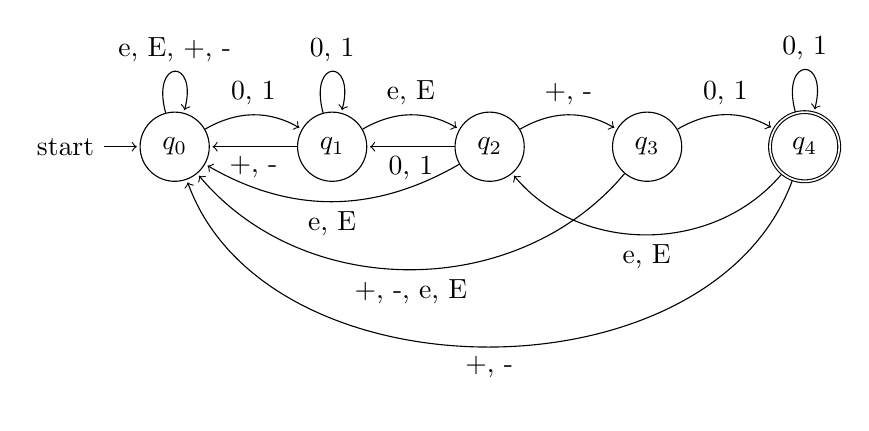
\begin{tikzpicture}[shorten >=1pt,node distance=2cm,on grid,auto] 
        \node[state,initial] (q_0)   {$q_0$}; 
        \node[state] (q_1) [right=of q_0] {$q_1$}; 
        \node[state] (q_2) [right=of q_1] {$q_2$}; 
        \node[state] (q_3) [right=of q_2] {$q_3$}; 
        \node[state, accepting] (q_4) [right=of q_3] {$q_4$}; 
        \path[->] 
            (q_0)
                edge [bend right=-30] node {0, 1} (q_1)
                edge [loop above] node {e, E, +, -} ()
            (q_1)
                edge [bend right=-30] node {e, E} (q_2)
                edge node {+, -} (q_0)
                edge [loop above] node {0, 1} ()
            (q_2)
                edge [bend right=-30] node {+, -} (q_3)
                edge node {0, 1} (q_1)
                edge [bend left=30] node {e, E} (q_0)
            (q_3)
                edge [bend right=-30] node {0, 1} (q_4)
                edge [bend left=50] node {+, -, e, E} (q_0)
            (q_4)
                edge [loop above] node {0, 1} ()
                edge [bend left=50] node {e, E} (q_2)
                edge [bend left=70] node {+, -} (q_0);
    \end{tikzpicture}
\end{homeworkProblem}

\pagebreak

\begin{homeworkProblem}
    Let \(A = \langle Q, \Sigma, \delta, q_0, F\rangle\) and \(B = \langle Q, \Sigma, q_0, F'\rangle\) be two
    nondeterministic finite automata such that \(F' = Q \setminus F\).

    Prove or disprove: The language of \(L(B)\) is the complement of the language
    \(L(A)\).

    \begin{figure}[here]
        \centering
        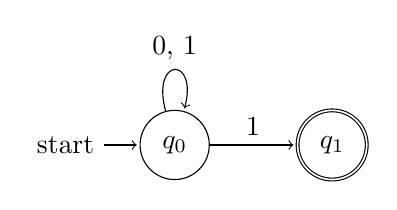
\begin{tikzpicture}[shorten >=1pt,node distance=2cm,on grid,auto] 
            \node[state, initial] (q_0)   {$q_0$}; 
            \node[state, accepting] (q_1) [right=of q_0] {$q_1$}; 
            \path[->] 
                (q_0)
                    edge node {1} (q_1)
                    edge [loop above] node {0, 1} ();
        \end{tikzpicture}
        \caption{Automata \(A\)}
        \label{fig:automataA}
    \end{figure}

    \begin{figure}[here]
        \centering
        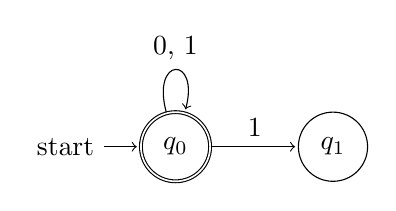
\begin{tikzpicture}[shorten >=1pt,node distance=2cm,on grid,auto] 
            \node[state, accepting, initial] (q_0)   {$q_0$}; 
            \node[state] (q_1) [right=of q_0] {$q_1$}; 
            \path[->] 
                (q_0)
                    edge node {1} (q_1)
                    edge [loop above] node {0, 1} ();
        \end{tikzpicture}
        \caption{Automata \(B\)}
        \label{fig:automataB}
    \end{figure}

    As a counterexample, consider the automata \(A\) and \(B\) pictured in Figure ~\ref{fig:automataA}
    and Figure ~\ref{fig:automataB} respectively.
    \\

    The only difference between the two automata is that the final state set of \(B\), \(F'\) is just \(F' = Q \setminus F\)
    where \(Q\) is the set of states in \(A\) and \(F\) is the set of final states in \(A\).
    \\

    This is a counterexample because the word \(\omega = 1\) is accepted by both automata.
    Thus \(\omega \in L(A)\) and \(\omega \in L(B)\) therefore \(L(A)\) is not the complement
    of \(L(B)\).
\end{homeworkProblem}

\end{document}
